\documentclass[]{article}
\usepackage{amssymb,amsmath}
\usepackage{ifxetex,ifluatex}
\usepackage{fixltx2e} % provides \textsubscript
\usepackage{float} % provides the H option for float placement
\usepackage{graphicx}
\ifxetex
  \usepackage{fontspec,xltxtra,xunicode}
  \defaultfontfeatures{Mapping=tex-text,Scale=MatchLowercase}
  \newcommand{\euro}{€}
\else
  \ifluatex
    \usepackage{fontspec}
    \defaultfontfeatures{Mapping=tex-text,Scale=MatchLowercase}
    \newcommand{\euro}{€}
  \else
    \usepackage[utf8]{inputenc}
  \fi
\fi
\usepackage{url}
\ifxetex
  \usepackage[setpagesize=false, % page size defined by xetex
              unicode=false, % unicode breaks when used with xetex
              xetex,
              bookmarks=true,
              pdfauthor={},
              pdftitle={},
              colorlinks=true,
              urlcolor=blue,
              linkcolor=blue]{hyperref}
\else
  \usepackage[unicode=true,
              bookmarks=true,
              pdfauthor={},
              pdftitle={},
              colorlinks=true,
              urlcolor=blue,
              linkcolor=blue]{hyperref}
\fi
\hypersetup{breaklinks=true, pdfborder={0 0 0}}
\setlength{\parindent}{0pt}
\setlength{\parskip}{6pt plus 2pt minus 1pt}
\setlength{\emergencystretch}{3em}  % prevent overfull lines
\setcounter{secnumdepth}{0}
\usepackage[vmargin=1in,hmargin=1in]{geometry} 


\begin{document}

\section{Assessing the suitability of forest inventories for basis of
spatial conservation prioritization}

Joona Lehtomäki\textsuperscript{1,2*} Sakari Tuominen\textsuperscript{3}
and Antti Leinonen\textsuperscript{4}

1 Department of Biosciences, P.O. Box 65 (Viikinkaari 1), FI-00014
University of Helsinki, Finland\\2 Finnish Environment Institute,
Natural Environment Centre, P.O. Box 140 (Mechelininkatu 34a), FI- 00251
Helsinki, Finland\\3 Finnish Forest Research Institute
(Metsäntutkimuslaitos), Vantaa, Finland\\4 The Finnish Forest Centre
(Suomen Metsäkeskus), Kajaani, Finland\\* Corresponding author

\textbf{Contact:}\\joona.lehtomaki@helsinki.fi, tel.
+358-9-191-57714\\sakari.tuominen@metla.fi\\antti.leinonen@metsakeskus.fi

\textbf{Journal:}\\Scandinavian Journal of Forest Research

\textbf{Type of paper:}\\Original research paper

\textbf{Running title:}\\Validation of spatial conservation
prioritization

\textbf{Manuscript statistics:}\\* word count (total) = xxx\\* figures =
xxx of which xxx in color\\* tables = xxx\\* references = xxx

\subsection{Abstract:}

In most parts of Fennoscandia, Boreal forest landscapes are primarily
managed for forestry purposes, but multi-objective planning including
biodiversity conservation is becoming more common. Often primary
biodiversity data, such as detailed distribution data for species, is
not available for defining conservation priorities over large areas. In
sharp contrast, data collected for forestry planning are frequently
available on various structural forest characteristics such as standing
tree volume, species composition and soil fertility. For conservation
planning purposes, data has to be 1) relevant for the planning at hand,
2) spatially extensive enough, 3) detailed enough, and 4) generally
available. Here, we demonstrate how to define conservation priorities in
a Finnish boreal forest landscape using national forest inventory data
sets. Inventoried data on forest characteristics such as tree volume,
average diameter, species composition, and soil fertility were used to
create proxy indexes for conservation value. These indexes were then
used as input for Zonation -- a method and software for spatial
conservation prioritization. Conservation priorities are often generated
without explicit considerations on how well the results capture the
distribution of conservation value. Here, we assess the validity of
Zonation results by a comparison to a number of independent data sets
that describe the distributions of features relevant for conservation,
such as existing protected areas and woodland key-habitats. We found
that prioritization based on forest inventory data can indeed produce
results that are informative for conservation. Regions on known high
conservation value were consistently identified by Zonation as high
priority areas. The process described here and the results produced by
these analyses feed directly into operational forest management by the
Finnish Forestry Center (Suomen Metsäkeskus). Similar analyses could be
implemented also in other regions of the boreal zone.

Keywords: adaptive management; conservation planning; forest
conservation management; spatial conservation prioritization; Zonation
software

\subsection{1. Introduction}

\subsubsection{1.1 Operational conservation planning in the forest
context (REF)}

\begin{itemize}
\item
  Boreal zone: Major ecoregion with very large geographic extent
  (Elbakidze et al. 2013)
\item
  Although among the least threatened of ecoregions (REF, IUCN?)

  \begin{itemize}
  \itemsep1pt\parskip0pt\parsep0pt
  \item
    Species have become threatened locally (Rassi et al. 2010)
  \item
    There is opportunity to set aside and/or manage relatively large
    areas of forest (Elbakidze et al. 2013)
  \item
    Significant role in carbon sequestration (Bradshaw et al. 2009)
  \end{itemize}
\item
  Conservation planning as a part of forestry management:

  \begin{itemize}
  \itemsep1pt\parskip0pt\parsep0pt
  \item
    Multi-citeria decision making (MCDM) (Kangas et al. 2005):
    Technically forest management planning, but can include components
    for biodiversity conservation as well.
  \item
    TRIAD (Côté et al. 2010): Functional zoning in forest management
    planning, different ``zones'' produces different outcomes
    (e.g.~conservation and timber)
  \item
    New management regimes (Kuuluvainen \& Grenfell 2012): Natural
    disturbance emulation (or ``continuous-cover forestry'') another way
    of bringing ``soft values'' to operative forestry management.
  \item
    Spatiotemporal dynamics (Leroux \& Rayfield 2013; Mönkkönen et al.
    2014): Important, but demanding to take into account. Many of the
    actual optimization methods cannot handle very large data.
  \item
    Need for change of how forest conservation is planned and
    implemented (Hanski 2011): A core network of protected areas
    surrounded by areas managed less intensively (``management
    landscapes'').
  \end{itemize}
\item
  Forest conservation planning needs to integrate closely with the
  existing land use planning and resource use planning (Ferrier \&
  Wintle 2009)
\item
  Successful integration largely depends on whether existing data that
  are already part of forestry planning can be utilized in conservation
  planning (REF) and on whether the results of conservation
  prioritization can be used in tools already existing in different
  administrative and management institutions (REF)

  \begin{itemize}
  \itemsep1pt\parskip0pt\parsep0pt
  \item
    In Finland, the decision-making context is a mixture of top-down and
    bottom-up action and different governance processes (Paloniemi \&
    Tikka 2008)
  \item
    Introduction to METSO-programme in Finland: aims, schedule, used
    tools with emphasis in ESMK (REF)
  \end{itemize}
\end{itemize}

\subsubsection{1.2 Spatial conservation prioritization}

\begin{itemize}
\item
  General description of background, methods, and worflows from
  (Lehtomäki \& Moilanen 2013)
\item
  Has been done in also in the boreal forest context (Mikusiński et al.
  2007; Lehtomäki et al. 2009; Sirkiä et al. 2012)⁠
\item
  Associated uncertainties often high , performance and efficiency
  unknown (Langford et al. 2011), need for (on-the-ground) validation
\item
  Objective of a spatial prioritization analysis can (and indeed often
  should) be not the \emph{highest} conservation priorities, but the
  \emph{lowest}. These are areas most suitable for e.g.~intensive
  forestry without being too harmful for biodiversity.
\item
  Usefulness of the results also depends on the sensitivity of the
  results. Particularly, if the informative part of the results
  (i.e.~the best fraction of the landscape for e.g.~conservation) is
  small relative to the overall size of the landscape then the results
  may very sensitive to various factors
\end{itemize}

\subsubsection{1.3 Data issues}

\begin{itemize}
\item
  Reliable and extensive data on species occurrence is rarely available,
  but not in the case of Finnish forest (REFS, check the flying squirrel
  / polypore papers): What to use as a surrogate?
\item
  Using forest inventory data as a basis for conservation prioritization
  is effectively using surrogates for the primary forest biodiversity
  data (species and habitats occurrence data)
\item
  Building the ecological model through expert elicitation is a widely
  used technique (REFS)
\item
  Habitat Suitability Indexes (HSI) another widely adopted approach
  (something by Kouki et al.)
\end{itemize}

\subsubsection{1.4 Aims and scope of the paper}

\begin{enumerate}
\def\labelenumi{\arabic{enumi}.}
\itemsep1pt\parskip0pt\parsep0pt
\item
  Investigate whether commonly available forestry data sets are a useful
  basis for spatial conservation prioritization

  \begin{itemize}
  \itemsep1pt\parskip0pt\parsep0pt
  \item
    The nature of the data (MSNFI vs.~more detailed data).

    \begin{itemize}
    \itemsep1pt\parskip0pt\parsep0pt
    \item
      MSNFI is a continuous estimate that is more accurate and unbiased
      over larger extents (Tomppo 2006)
    \item
      Stand-based inventory data more accurate, but this will depend on
      the age of the data. Additionally there is an unknown quantity of
      variation caused by differences between practitioners.
    \end{itemize}
  \item
    Technical usability of the data

    \begin{itemize}
    \itemsep1pt\parskip0pt\parsep0pt
    \item
      Usually well managed and relatively easy to work with
    \item
      MSNFI expandable beyond the standard products (i.e.~segmentation
      provided by Sakari)
    \item
      Legal issues may restrict usability
    \end{itemize}
  \item
    Adequacy of data in the construction of the ecological model

    \begin{itemize}
    \itemsep1pt\parskip0pt\parsep0pt
    \item
      What attributes of fores inventory data can be used for defining
      conservation value (largely based on expert views)?
    \end{itemize}
  \end{itemize}
\item
  Investigate how well spatial conservation prioritization (using forest
  inventory data and Zonation) can inform conservation decision-making
  in operational forestry planning in Finland

  \begin{itemize}
  \itemsep1pt\parskip0pt\parsep0pt
  \item
    Comparison of the results to a set of independent data sets
  \item
    What are the advantages/disadvantages of different scales?

    \begin{itemize}
    \itemsep1pt\parskip0pt\parsep0pt
    \item
      Being part of operational planning implies very fine-scale (maybe
      Kangas et al. 2014?)
    \item
      On the other hand, large scale will even out the potential errors
      (Tomppo 2006)
    \end{itemize}
  \end{itemize}
\item
  Suggest ways to improve use of spatial conservation prioritization
  methods in operational forestry planning (Not necessarily an aim in
  itself, will be part of the discussion anyway)

  \begin{itemize}
  \itemsep1pt\parskip0pt\parsep0pt
  \item
    Importance of monitoring which can also be done as a part of
    standard forestry operations
  \item
    How to improve data? How to improve analyses?
  \end{itemize}
\end{enumerate}

\subsection{2. Material and methods}

\subsubsection{2.1 Data for spatial conservation prioritization and its
validation}

\begin{itemize}
\item
  Data used for this purpose must be available across the entire study
  area, not from individual locations only. Source of the data matters
  as different data sets have different levels of uncertainty etc.
\item
  Prioritization data sets (ESMK + LTI inventories + segmented MSNFI)

  \begin{itemize}
  \itemsep1pt\parskip0pt\parsep0pt
  \item
    Brief description of the data used
  \item
    \textbf{Table 1:} Data sets used for the construction of the
    ecologically based model and index of conservation value (see 2.3
    for explanation).
  \end{itemize}
\item
  Validation data (PAs + woodland key-habitats + METSO-deals + ENGO
  sites (?))

  \begin{itemize}
  \itemsep1pt\parskip0pt\parsep0pt
  \item
    \textbf{Table 2:} Additional data used for the independent
    validation of results
  \end{itemize}
\end{itemize}

\subsubsection{2.2 The ecological model}

\begin{itemize}
\item
  Short description here, more detailed in the supplement
\item
  What is: a conceptual model for conservation prioritization

  \begin{itemize}
  \itemsep1pt\parskip0pt\parsep0pt
  \item
    In this context, ``ecological model'' means a conceptual model that
    converts whatever data we have into something meaningful from the
    perspective of conservation
  \item
    The reasoning for translating the information on forest structural
    features to something important for conservation (REF)
  \end{itemize}
\item
  Data selection by experts (supl.)
\item
  Benefit functions (supl.)

  \begin{itemize}
  \itemsep1pt\parskip0pt\parsep0pt
  \item
    Justification behind using the benefit functions
  \end{itemize}
\item
  Weighting of features and connectivity (supl.)

  \begin{itemize}
  \itemsep1pt\parskip0pt\parsep0pt
  \item
    Based on discussions with the experts + web questionnaire
  \item
    \textbf{Figure 1:} The ecological model. Data sets, the structure of
    the index + the selected connectivity distances and connectivity
    interaction types. (similar to (Sirkiä et al. 2012)⁠)
  \end{itemize}
\end{itemize}

\subsubsection{2.4 Analysis variants}

\begin{itemize}
\item
  We selected four analysis variants XXX in order to examine a suite of
  scenarios directly relevant for the planning need.
\item
  \textbf{Table 3:} Analysis variants. (link to Fig 1)
\end{itemize}

\subsubsection{2.5 Interpretation of results (prioritity rank maps)}

\begin{itemize}
\itemsep1pt\parskip0pt\parsep0pt
\item
  Spatial prioritization

  \begin{itemize}
  \itemsep1pt\parskip0pt\parsep0pt
  \item
    Priority rank maps for the four variants of Table (3)
  \item
    Representation level boxplots for particular feature groups (by tree
    spp or fertility?) for particular top fraction of the landscape;
    This particular top fraction could correspond to the overall area
    objective for ESMK (will have to check what it is)
  \end{itemize}
\item
  Comparison of variants

  \begin{itemize}
  \itemsep1pt\parskip0pt\parsep0pt
  \item
    Operationally, how robust are the results? i.e.~depending on which
    variant is used, where are highest priorities? Also, what's the
    effect of the ``top fraction of the landscape'' selected?
  \item
    Overlap and correlations using Kendall Tau and Jaccard index (needs
    an extra Figure?)
  \end{itemize}
\item
  Validation with independent data sets

  \begin{itemize}
  \itemsep1pt\parskip0pt\parsep0pt
  \item
    Distributions of the rank priorities using a given comparison data
  \item
    Other stats (mean, SD, range?) of priorities within comparison data
  \item
    Comparison to the data (indexes) that the prioritization is based on
    (Supl?)
  \end{itemize}
\end{itemize}

\subsection{3.Results}

\subsubsection{3.1 Spatial priorities}

\begin{itemize}
\item
  \textbf{Figure 2:} Priority rank maps for analysis variants (all 4).
\item
  \textbf{Figure 3:} representation levels of feature groups (grouped by
  spp or fertility) for top fraction of the landscape
\item
  Priorities tend to be lower on areas with data source XXX\ldots{}
  (probably MSNFI)
\item
  General patterns are strongly affected by the connectivity components
  included, but this is scale dependent
\end{itemize}

\subsubsection{3.2 Comparison of variants}

\begin{itemize}
\item
  \textbf{Table 4:} Summary statistics on the differences between the
  variants at given levels of the top fraction of the landscape:
  overlap.
\item
  The results show that the absolute highest fraction of the landscape
  relatively independent to which variant is used.
\item
  Incorporating connectivity components will result in tradeoffs:
  accounting for the connectivity to existing protected areas aggregate
  priorities near conservation areas and draw them away from locations
  further away
\end{itemize}

\subsubsection{3.3 Comparison to independent data sets}

\begin{itemize}
\item
  \textbf{Figure 4:} Distributions of priority ranks (histograms) in
  different, independent data sets.
\item
  Characteristics of individual data sets determine which variant should
  be compared to which data. E.g. the inventory data collected by the
  conservation NGOs should be compared to the variant that accounts for
  the connectivity to existing protected areas - because this was a
  specific objective in data collection.
\end{itemize}

\subsection{4. Discussion}

\begin{itemize}
\itemsep1pt\parskip0pt\parsep0pt
\item
  Comparison to independent data sets relevant for biodiversity
  conservation indicate that known valuable locations indeed emerge from
  the analysis with high priorities +Data from conventional forestry
  planning coupled with a spatial conservation prioritization tool like
  Zonation can be used to identify areas of high conservation priorities

  \begin{itemize}
  \itemsep1pt\parskip0pt\parsep0pt
  \item
    Characterize how the validation worked or not with different data
    sets
  \item
    Note that results should not be extrapolated beyond the current
    problem definition
  \item
    Depending on the prioritization tool used, the analysis and the
    results often are static → if and when dynamics are not considered
    it is hard to say much about persistence and hence effectiveness.
  \item
    Formulation of the objectives is thus important and the results
    should not extrapolated beyond the scope of the analysis at hand
  \end{itemize}
\item
  Aligning planning needs, spatial scale, resolution and the (planning)
  decision-making context need careful consideration

  \begin{itemize}
  \itemsep1pt\parskip0pt\parsep0pt
  \item
    There is no single best solution: the most suitable solution will
    have to be carefully planned
  \item
    This implies that operational capacity also needs to be in place in
    order for the analysis be repeatable and adaptive
  \item
    Learning institutions, enabling and empowerment important for the
    long-term adoption of new techniques (refs Knight etc.)
  \end{itemize}
\item
  Incorporation of the results into operational forestry planning --
  ``the manager's view''

  \begin{itemize}
  \itemsep1pt\parskip0pt\parsep0pt
  \item
    Antti
  \end{itemize}
\item
  Opportunities for improvement:

  \begin{itemize}
  \itemsep1pt\parskip0pt\parsep0pt
  \item
    Data

    \begin{itemize}
    \itemsep1pt\parskip0pt\parsep0pt
    \item
      There are clear differences in the quality of the data
    \item
      How to improve the data base underlying prioritizations, noting
      that data needs to be available across a large area?
    \item
      What would be ideal data for validation?
    \end{itemize}
  \item
    Methods

    \begin{itemize}
    \itemsep1pt\parskip0pt\parsep0pt
    \item
      More realistic ecological models accounting for X, XX, and XXX
    \item
      Known planning needs that this analysis does not answer.
    \end{itemize}
  \item
    Enabling input to decision-making
  \end{itemize}
\item
  Mainstreaming the methods

  \begin{itemize}
  \itemsep1pt\parskip0pt\parsep0pt
  \item
    The road forward
  \end{itemize}
\end{itemize}

\section{References}

Bradshaw, C. J. a, I. G. Warkentin, and N. S. Sodhi. 2009. Urgent
preservation of boreal carbon stocks and biodiversity.. Trends in
Ecology and Evolution \textbf{24}:541--8. Retrieved from
\url{http://dx.doi.org/10.1016/j.tree.2009.03.019}.

Côté, P., R. Tittler, C. Messier, D. D. Kneeshaw, A. Fall, and M.-J.
Fortin. 2010. Comparing different forest zoning options for
landscape-scale management of the boreal forest: Possible benefits of
the TRIAD. Forest Ecology and Management \textbf{259}:418--427.
Retrieved from
\url{http://linkinghub.elsevier.com/retrieve/pii/S0378112709007804}.

Elbakidze, M., P. Angelstam, N. Sobolev, E. Degerman, K. Andersson, R.
Axelsson, O. Höjer, and S. Wennberg. 2013. Protected area as an
indicator of ecological sustainability? A century of development in
Europe's boreal forest. Ambio \textbf{42}:201--14. Retrieved from
\url{http://dx.doi.org/10.1007/s13280-012-0375-1}.

Ferrier, S., and B. A. Wintle. 2009. Quantitative Approaches to Spatial
Conservation Prioritization: Matching the Solution to the Need. Page 304
in A. Moilanen, K. A. Wilson, and H. P. Possingham, editors. Spatial
Conservation Prioritization: Quantitative Methods \& Computational
Tools. Oxford University Press, Oxford.

Hanski, I. 2011. Habitat loss, the dynamics of biodiversity, and a
perspective on conservation. Ambio \textbf{40}:248--255. Retrieved from
\url{http://www.springerlink.com/index/10.1007/s13280-011-0147-3}.

Kangas, J., R. Store, and A. Kangas. 2005. Socioecological landscape
planning approach and multicriteria acceptability analysis in
multiple-purpose forest management. Forest Policy and Economics
\textbf{7}:603--614. Retrieved from
\url{http://linkinghub.elsevier.com/retrieve/pii/S1389934104000024}.

Kuuluvainen, T., and R. Grenfell. 2012. Natural disturbance emulation in
boreal forest ecosystem management - theories, strategies, and a
comparison with conventional even-aged management. Canadian Journal of
Forest Research \textbf{1203}:1185--1203.

Langford, W. T., A. Gordon, L. Bastin, S. Bekessy, M. D. White, and G.
Newell. 2011. Raising the bar for systematic conservation planning.
Trends in Ecology and Evolution \textbf{26}:634--640. Retrieved from
\url{http://linkinghub.elsevier.com/retrieve/pii/S0169534711002333}.

Lehtomäki, J., E. Tomppo, P. Kuokkanen, I. Hanski, and A. Moilanen.
2009. Applying spatial conservation prioritization software and
high-resolution GIS data to a national-scale study in forest
conservation. Forest Ecology and Management \textbf{258}:2439--2449.
Retrieved from
\url{http://linkinghub.elsevier.com/retrieve/pii/S0378112709005969}.

Lehtomäki, J., and A. Moilanen. 2013. Methods and workflow for spatial
conservation prioritization using Zonation. Environmental Modelling \&
Software \textbf{47}:128--137. Retrieved from
\url{http://linkinghub.elsevier.com/retrieve/pii/S1364815213001072}.

Leroux, S. J., and B. Rayfield. 2013. Methods and tools for addressing
natural disturbance dynamics in conservation planning for wilderness
areas. Diversity and Distributions \textbf{20}:1--14. Retrieved from
\url{http://doi.wiley.com/10.1111/ddi.12155}.

Mikusiński, G., R. L. Pressey, L. Edenius, H. Kujala, A. Moilanen, J.
Niemelä, and T. Ranius. 2007. Conservation planning in forest landscapes
of fennoscandia and an approach to the challenge of countdown 2010.
Conservation Biology \textbf{21}:1445--1454.

Mönkkönen, M., A. Juutinen, A. Mazziotta, K. Miettinen, D. Podkopaev, P.
Reunanen, H. Salminen, and O.-P. Tikkanen. 2014. Spatially dynamic
forest management to sustain biodiversity and economic returns. Journal
of environmental management \textbf{134C}:80--89. Retrieved from
\url{http://www.ncbi.nlm.nih.gov/pubmed/24463852}.

Paloniemi, R., and P. M. Tikka. 2008. Ecological and social aspects of
biodiversity conservation on private lands. Environmental Science \&
Policy \textbf{11}:336--346. Retrieved from
\url{http://linkinghub.elsevier.com/retrieve/pii/S1462901107001256}.

Rassi, P., E. Hyvärinen, A. Juslén, and I. Mannerkoski. 2010. The 2010
Red List of Finnish species. Helsinki.

Sirkiä, S., J. Lehtomäki, H. Lindén, E. Tomppo, and A. Moilanen. 2012.
Defining spatial priorities for capercaillie Tetrao urogallus lekking
landscape conservation in south-central Finland. Wildlife Biology
\textbf{18}:337--353.

Tomppo, E. O. 2006. The Finnish multi-source National Forest Inventory -
small area estimation and map production. Pages 195--224 in A. Kangas
and M. Maltamo, editors. Forest inventory. Methodology and Applications.
Dordrecht, Germany. Retrieved from \url{Springer}.

\section{Tables}

\section{Figures}

\textbf{Figure 1.} Schematics of the analysis setup. Different parts of
the analysis were done in different software environments (see text).
Analysis feature layers (index layers) were constructed from 3 different
data sources (Table 1 and a condition layer (see text) was applied on
all of them. Different Zonation analysis variants are indicated by
arrows 1-4 (see Table 3) with closed circles indicating the analysis
features used. Each analysis variant resulted in a priority maps (Figure
2) and feature-specific performance curves (Figure 3). For validation
purposes, each rank priority map was compared to a set of independent
validation data to determine the mean and the distribution of ranks
(Figure 4).

\textbf{Figure 2.} Conservation rank priority maps.

\textbf{Figure 3.} Performance curves for variant XXX (REPLACE
``PERFORMANCE CURVES'')

\textbf{Figure 4.} Distribution of rank priorities in comparison data
sets.

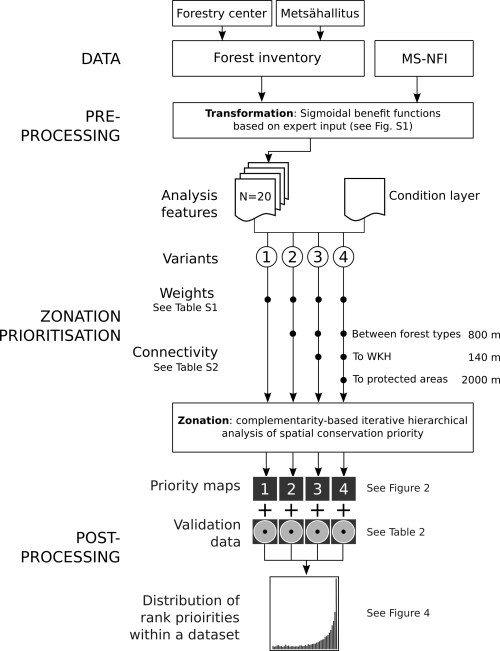
\includegraphics{figs/Fig1_w500.png}\\\textbf{Figure 1:} Schematics of
the analysis setup.

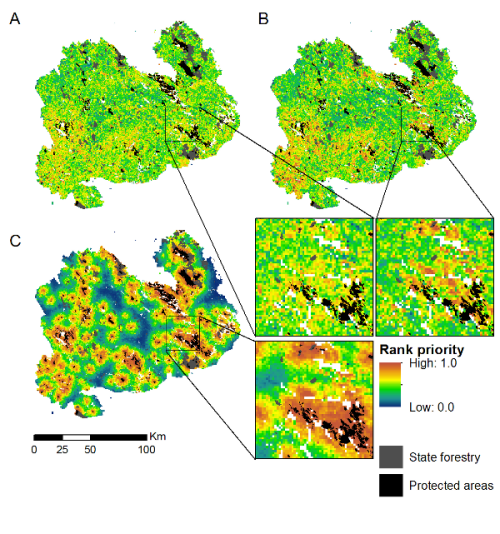
\includegraphics{figs/Fig2_w500.png}\\\textbf{Figure 2:} Conservation
rank priority maps.

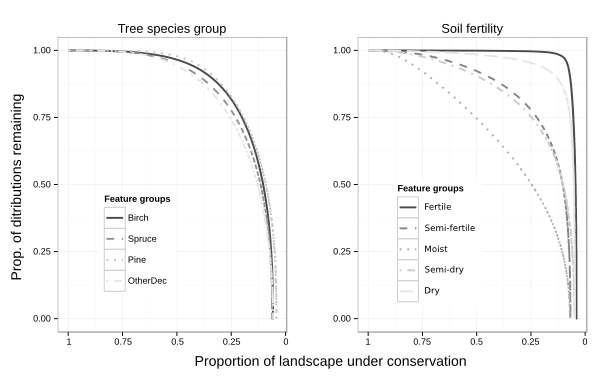
\includegraphics{figs/Fig3_w600.png}\\\textbf{Figure 3:} Performance
curves.

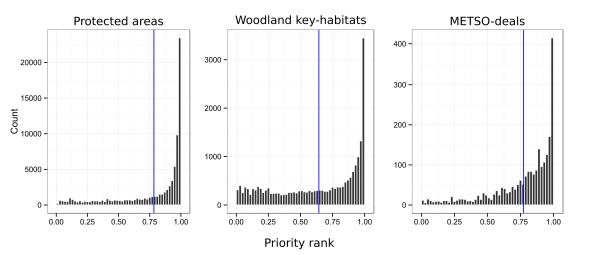
\includegraphics{figs/Fig4_w600.png}\\\textbf{Figure 4:} Rank histograms
for validation data sets.

\clearpage

\section{Supplementary material}

Building the ecological model Expert elicitation Figure S1: The benefit
functions used to scale the perceived, expert opinion based conservation
value (y-axis) to forest structural characteristics (x-axis)
Segmentation of the MSNFI data

Analysis setup: Table S1: Feature weights Table S2: Connectivity matrix

\end{document}
